The design of the software, architecture, and technologies used to create the web-application and databases are described in the following section. The analysis being performed by the web-application and how it performs each analysis is discussed and how the back end queries each database.

\subsection{Database Technologies}

This section covers the underlying technologies used to implement the databases being benchmarked. This is important to note in terms of how portable each technology is, how difficult the configuration is before each database can be used for a given project, or limitations on performance or hardware requirements due to software requirements. While each database technology has varying capabilities, in terms of being supported for a given operating system, they each provide support for being deployed in a Docker container.

\subsubsection{PostgreSQL}
PostgreSQL is written in the C programming language, is an object-oriented relational database, and is queried via SQL commands. PostgreSQL, like many relational databases, is ACID-compliant and robust to transactional failures. It is built to be extensible with a variety of extensions one can install for additional features such as UUID or spatial indexing. PostgreSQL can deploy on a variety of major operating systems such as Windows, Mac, Linux (Redhat, Debian, and a few others), Solaris, and BSD.

This product is mature and has a large amount of support, especially from its open-source community. Postgres is flexible in that it supports a variety of data types and allows one to define one's own. Founder of NewsBlur\footnote{\url{https://newsblur.com/}}, Samuel Clay, mentions using Postgres for multiple years for storing millions of sites and subscriptions. Canonical\footnote{\url{https://canonical.com/}} founder, Mark Shuttleworth, explains that, while using Postgres during the development of Launchpad, finding it ``robust, fast, and professional in every regard'' \cite{postgres-about}.

Many of these features and opinions of using PostgreSQL in production environments on this scale is why PostgreSQL was the database of choice to benchmark against.

\subsubsection{JanusGraph}

JanusGraph is a highly scalable graph database that is ready to be clustered among multiple machines. It is a transactional database which supports ACID-compliance and eventual consistency \cite{janusgraph-main}. It is written in Java and in thus platform independent. JanusGraph is a project under The Linux Foundation and is forked from the Titan project as a continuation of the vision in creating an open-source, scalable, highly concurrent graph database. There is support for those wishing to migrate from Titan in order to benefit from the bug fixes and additional features now supported via JanusGraph \cite{janusgraph-titan}.

JanusGraph is largely based on the Apache tech-stack making use of technologies such as Apache TinkerPop, Lucene, Cassandra, Hadoop, and more. Gremlin is the native language through which JanusGraph is queried but, as mentioned in Section \ref{subsec:lang}, can be extended for Cypher queries. The property graph model is used, benefits from optional support for advanced search capabilities, and having no-single point of failure \cite{janusgraph-docs}.

\begin{figure}[h!]
    \centering
    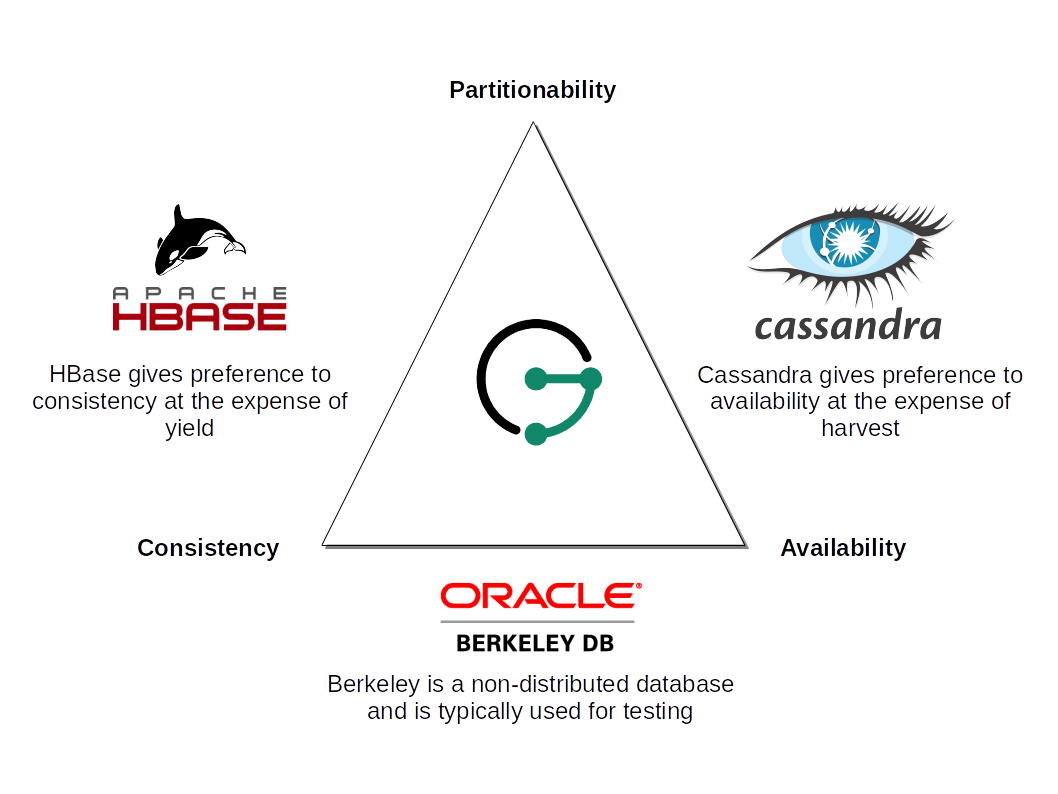
\includegraphics[width=10cm]{img/CAP-JanusGraph.png}
    \caption{The CAP theorem illustrated using JanusGraph's three supporting storage back ends. This diagram is largely inspired from Chapter 1 in Titan's documentation and is adjusted for JanusGraph \cite{titan-cap}.}
    \label{fig:janusgraph-cap}
\end{figure}

JanusGraph can store graph data via three supporting back ends; Apache Cassandra, Apache HBase, and Apache Berkeley. The CAP Theorem (Section \ref{cap}) should be referred to when considering which of the three back ends to use -- this is illustrated in Figure \ref{fig:janusgraph-cap}.

Examples of companies who have deployed JanusGraph in production include Netflix, Redhat, Uber, and IBM \cite{janusgraph-readme}. The professional support, documentation, and fact that one is able to leverage all these advanced features for free is why JanusGraph is one of the graph databases used in this investigation. The configuration of JanusGraph used in this report is with Apache Cassandra as the storage back end and ElasticSearch as the search engine for spatial and temporal query support.

\subsubsection{TigerGraph}

TigerGraph is an enterprise level graph analytics platform developed in the C++ programming language. TigerGraph was developed with hindsight from projects such as Apache TinkerPop and Neo4j and provides features such as native parallel graph processing and fast offline batch loading to get the edge against its competitors \cite{tigergraph-benchmark} \cite{conference-trip}. Unlike JanusGraph, TigerGraph was developed from scratch in order to effectively create the next generation of graph database technology. TigerGraph won Strata Data’s ``Most Disruptive Startup'' Award for its breakthrough in this regard \cite{tigergraph-award}.

Some of the use cases explicitly mentioned by TigerGraph\footnote{\url{https://www.tigergraph.com/solutions/}} is geospatial and time series analysis. This lends itself as a promising database technology for this investigation. TigerGraph is queried using their GSQL querying language (see Section \ref{subsec:lang}) where queries are optimized via an installation process where a REST endpoint is also generated in the process. Like JanusGraph, TigerGraph can be deployed on multi-machine clusters but this is limited to the enterprise version of this product. TigerGraph uses Apache Zookeeper for Kafka cluster management and Apache Kafka for message queuing.

GraphStudio is a web interface which is packaged along with TigerGraph which provides an interface to write, install and visualize queries, design and export one's graph schema, and monitor database performance. This makes use of an Nginx web server \cite{tigergraph-infoworld}.

For all intents and purposes, the developer edition is more than capable to perform the investigation of this paper.

\subsection{Web-application Simulation}
The web-application, called Providentia\footnote{The name of the web-application is a nod to JanusGraph and Titan's theme of Roman mythology. Providentia is associated with provision and forethought \cite{providentia-meaning}. This was thought to be fitting due to the nature of the experiments bringing out the best database to move forward with when making a decision on which technology to use for storing and modeling one's data.}, is used to queue analysis into a pipeline where each benchmark is to be run, server performance measured, and accumulated results to be displayed. This is deployed on target hardware and will import a subset of the data (given a configurable percentage) and then one will be able to use the web-based interface to perform all necessary benchmarking tasks.

The architecture and how each technology communicates is illustrated in Figure \ref{fig:providentia-architecture}. The databases are containerized using Docker\footnote{\url{https://www.docker.com/}}.

\begin{figure}[h!]
    \centering
    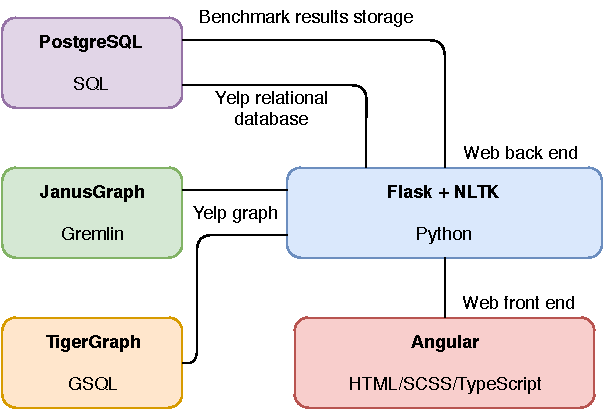
\includegraphics[width=10cm]{img/providentia-architecture.pdf}
    \caption{The architecture of Providentia.}
    \label{fig:providentia-architecture}
\end{figure}

JanusGraph has some Java specific features that add limitations when making use of embedded Gremlin in Python. These limitations are when trying to make use of mixed indexing search predicates such as spatial queries. The workaround for this was making use of the Gremlin Translator which would take Gremlin as a string and interpret it on the server side.

The first motivation towards using a Python back end is that the text in the reviews can be analysed using NLTK for easy sentiment analysis. The second is that a simple REST API can easily and quickly be designed using the Flask framework. Angular was subjectively chosen as the front end framework as it allows for fast and stable front end web development. All benchmark results are stored in a separate database within PostgreSQL.

The front end of Providentia allows a user to query each database, test the sentiment classifier, add benchmarking jobs and to review the performance and results of each analysis. Each job is run serially to avoid too much interference and competition between each database for resources. At intervals the CPU performance and memory consumption is measured and stored in PostgreSQL. The server performance and results of an analysis can be viewed together to validate that the outputs are the same and how each database uses the server's resources.

\subsection{Data Analysis}
Over each of the databases a number of data analysis jobs are performed on the data. This section describes what each analysis aims to do and how they align to a typical real world use case. Each of these jobs have some kind of spatiotemporal aspect to test the accessibility of the data to demonstrate how well the given database handles the data.

These analysis are run over different percentages of the data loaded in each database and the performance is then measured and discussed in Section \ref{sec:experiments}. This section goes into more detail about the types of queries written and how well each language expresses each
query.

\subsubsection{Sentiment Analysis}
One application for graph analytic platforms is in machine learning. In order to further build context around each of the kernels mentioned in the next section, a simple binary sentiment classifier is used to classify the text of reviews as representing either a positive or negative sentiment. Sentiment analysis is a class of natural language processing where subjective information is extracted from a given text \cite{sentiment-analysis-gupta}.

Although this investigation does not explore the applications of machine learning models on spatiotemporal data, it will explore how it could reveal interesting information alongside patterns among the data. All natural language processing is done using the Natural Language Toolkit (NLTK)
\footnote{\url{https://www.nltk.org/}} for Python.

\subsubsubsection{Machine Learning Model}
NLTK's Na\"ive Bayes classifier\footnote{\texttt{nltk.NaiveBayesClassifier}} was used as the model to train and classify sentiment. Na\"ive Bayes is a probabilistic machine learning model which has proven very effective in text classification. A limitation of this model on a binary classification problem include only being able to perform linear separability. This should not be an issue regarding the use of adjectives as feature vectors since the most informative adjectives seem to be verbose and particular to a specific sentiment e.g. words like horrible, disgusting, perfect, and wonderful \cite{rish2001empirical}. One risk is that of negation which may make certain adjectives less information e.g. good vs not good \cite{blanco2011some}. Nevertheless the model performs well in terms of separating the two classes and, given the training data, has a good generalization performance. \textcolor{blue}{TODO: Show results to justify this}

\subsubsubsection{Training Process}
The data used is from this dataset and is extracted with the following assumption -- 1 star reviews hold negative sentiment and 5 star reviews hold positive sentiment. 10 000 1 star reviews are tagged as ``negative'' and 10 000 5 star reviews are tagged as ``positive''. Training and validation data are split by 70\% training and 30\% validation.

The data pre-processing and training of the Na\"ive Bayes model used in this investigation is based on the process described by Munir \cite{SamiraMunir}. Using NLTK, one can separate different parts of speech within a given sentence or paragraph. First, a bag of words is created from both classes
the training data. For a given review, punctuation is removed, words are tokenized, stop words removed, and only adjectives are kept and these adjectives are added to our bag. A frequency distribution is then used to determine the most informative words for a given label.

The top 5000 occurring adjectives are kept in the bag. These informative words can be seen as 5000 attributes where a review has the value ``true'' under an attribute found in the text and ``false'' when a review does not have that attribute contained within its text. This will be how a feature set will be constructed for a review. A Python dictionary is constructed with these 5000 attributes as keys and their value as the respective state as a boolean. This is then the first element of a tuple and the tag is the second. A trivial example of a feature set can be seen in Figure \ref{fig:bog-attri}.

\begin{figure}[h!]
    \centering
    \begin{tabular}{ |p{2cm}|p{2cm}|p{2cm}|p{2cm}|p{2cm}|p{2cm}|}
        \hline
        \rowcolor{Gray}
        \multicolumn{6}{|c|}{Review Text}                                                                                                       \\
        \hline
        \multicolumn{6}{|c|}{I just ate the most yummy pizza at this restaurant! The setting was wonderful with outdoor seating on a patio}     \\
        \multicolumn{6}{|c|}{ with a beautiful view. Service was incredible and I felt safe in good hands!}                                     \\
        \hline
        \rowcolor{Gray}
        \multicolumn{6}{|c|}{Feature Set}                                                                                                       \\
        \hline
        \textbf{Horrible}         & \textbf{Dirty}                 & \textbf{Worst} & \textbf{Wonderful} & \textbf{Yummy} & \textbf{Perfection} \\
        \hline
        false                     & false                          & false          & true               & true           & false               \\
        \hline
        \rowcolor{LightGray}
        \multicolumn{1}{|c|}{Tag} & \multicolumn{5}{|c|}{Positive}                                                                              \\
        \hline
    \end{tabular}
    \vspace*{5mm}
    \caption{An example of a review tagged as positive with it's feature set.}
    \label{fig:bog-attri}
\end{figure}

All of the reviews are then processed into these feature sets and tagged then given to the model to learn. Once the model has been trained, a review is classified by breaking it up into a feature set, given to the model to classify and the predicted class label is then returned.

\subsubsection{Kernels}

\subsubsubsection{Kate's Restaurant Recommendation}
This analysis selects a user near the beginning of the dataset named Kate. This user has a number of reviews for restaurants in the Las Vegas area. A subset of reviews which hold a strictly greater than 3 star rating by Kate are selected and sorted by date descending in order to take the most relevant ones. These businesses are then selected, filtered by category ``Restaurants'', and other users who have an equal or greater than star rating are then selected as the recommending users.

Now assume that Kate has relocated to a new area. All businesses which have been rated strictly larger than 3 stars by the recommending users are then selected as restaurants to recommend to Kate in the new area. The text in these reviews are checked for sentiment and the percentage positive sentiment is displayed alongside the average star rating for each recommended restaurant. This sentiment vs. average star rating is used an interesting metric to analyse in terms of asking the question: How reliable is the star rating versus the actual sentiment found in the text?

The purpose of the first part of this kernel is to test the 1-hop graph traversal pattern. This hop is demonstrated in category filtering and finding users with mutual sentiment for a given review. This type of situation is faced by many recommendation technologies and this is quite a basic technique for recommendation. The additional challenge is the relocation of Kate and seeing how responsive the database is to the spatial and temporal aspect which is the second part of this kernel. The accumulated list of users is split into a separate query for each user to test the ability of each database technology to perform concurrent reads on subsets of data which is a strength of NoSQL databases.

\subsubsubsection{Review Trends in Phoenix 2018}
This analysis goes deeper into observing the trend of various characteristics of reviews versus their star ratings. This is a common analysis performed on the Yelp dataset \cite{yelp-trends-zhang} but the version in this investigation selects a subset of reviews only within the 2018 year in the Phoenix area. The spatiotemporal boundaries put on this subset may reveal hidden trends to look further into.

Reviews are extracted first by location (which results in a much smaller subset than extracting by date first) then by date. The reviews are then separated by star rating. For each star rating, the characteristics of ``funny'', ``useful'', and ``cool'' are accumulated and the text is classified as either positive or negative. For each star rating these are normalized and placed next to one another to see the characteristic of a review from each star group.

\subsubsubsection{\textcolor{blue}{ TODO: Come up with a third kernel.}}
\textcolor{blue}{ TODO: Discuss analysis simulation and language processing involved.}
